\chapter{Results \& Discussions}
\indent The results obtained from the cell balancing module and the MATLAB Simulink model are presented in form of graphs and figures. And observations made during testing are discussed in the chapter.



\section{Simulation results}
Initially the cells in pack are set at random SOC values so that pack is said to imbalanced. Simulation time is set for 15 hours and run in rapid accelerator mode in Simulink.


\begin{figure}[h!]
    \centering
    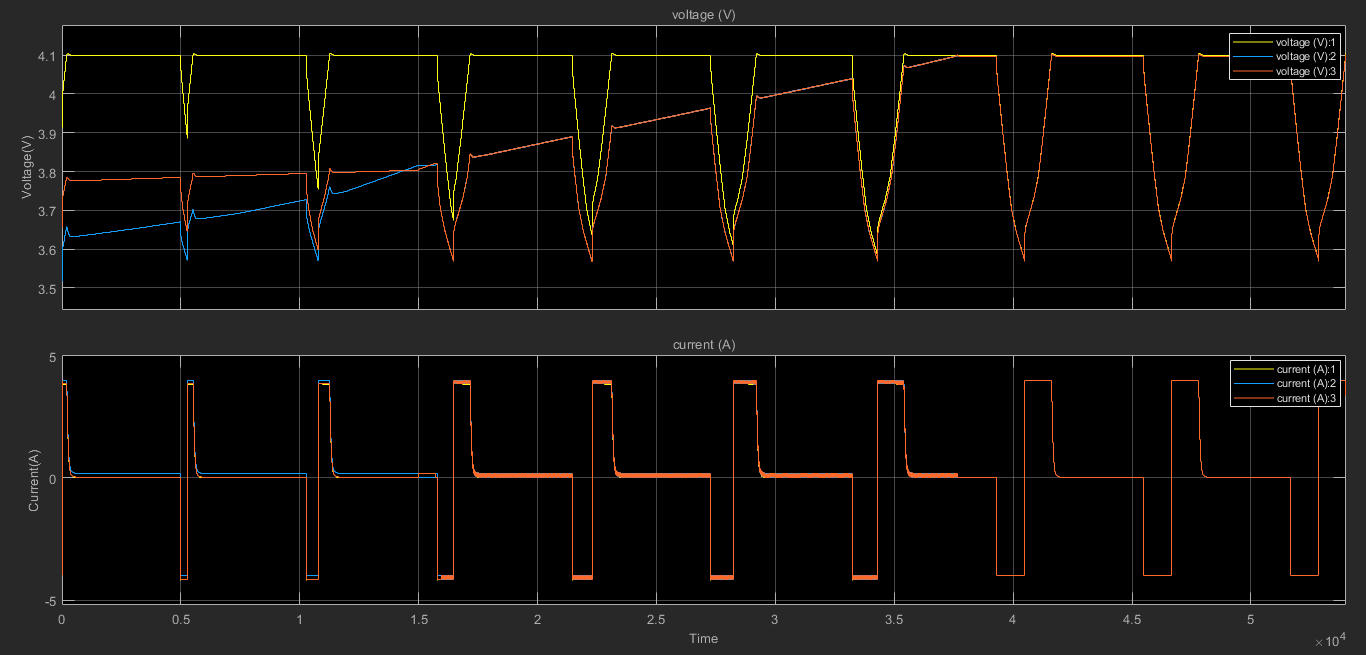
\includegraphics[scale = 0.5]{Chapter5/Figures/cellsVI.png}
    \caption{Cell voltage and current versus time during charge-discharge cycles}
\end{figure}

Fig 5.1 shows cell voltage and current versus time graph during charge-discharge cycles.Initially when battery pack is imbalanced the lowest voltage cell was limiting battery's full capacity even though other cells had charge remaining because of \acrshort{bms} cutting off discharge when one of the cell in pack reaches lowest set cell voltage in order to protect cells from  damage. As cell balancing algorithm kicks in cell voltages equalise and after 6 charge-discharge cycles the battery pack get balanced and deliver the rated capacity.
\vspace{0.5cm}
\begin{figure}[h!]
    \centering
    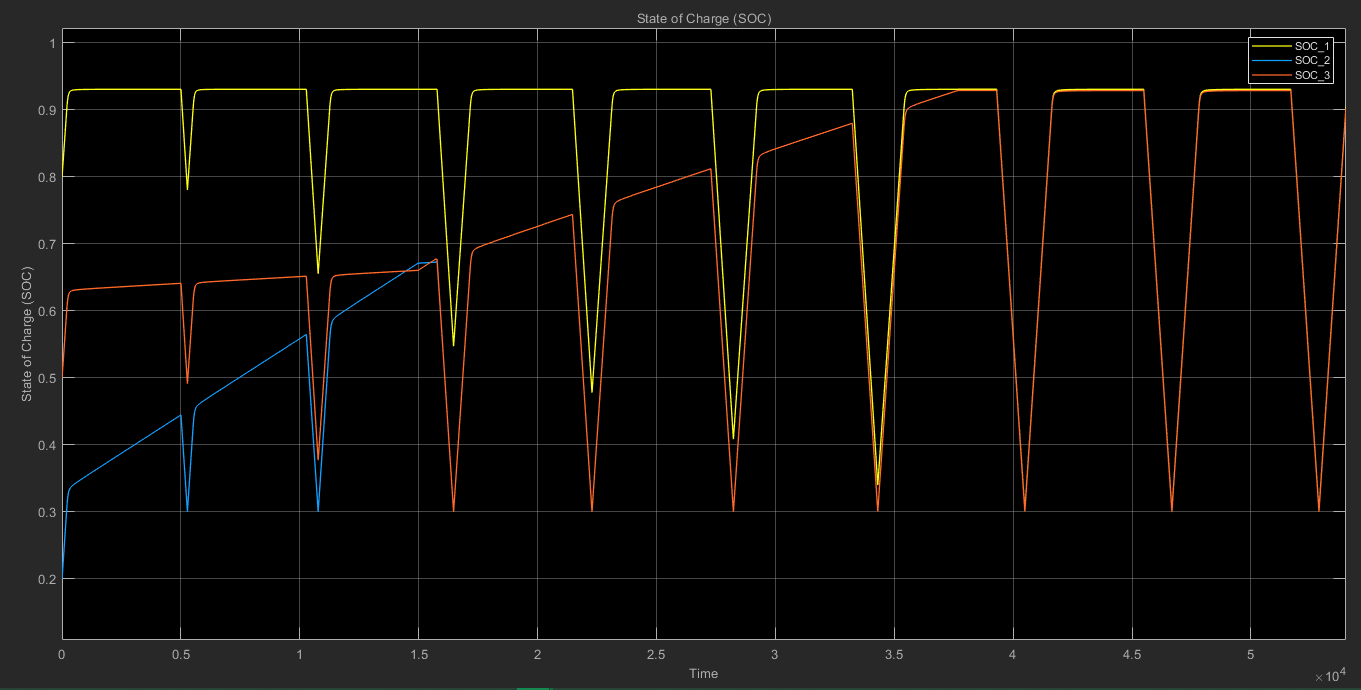
\includegraphics[scale = 0.5]{Chapter5/Figures/soc.png}
    \caption{State of charge of cells versus time during charge-discharge cycles}
\end{figure}

Figure 5.2 shows state of charge of cells versus time graph during charge-discharge cycles. Again it validates the circuit as by reporting full capacity utilisation after balancing circuit gradually equalise cell voltages.

\begin{figure}[h!]
    \centering
    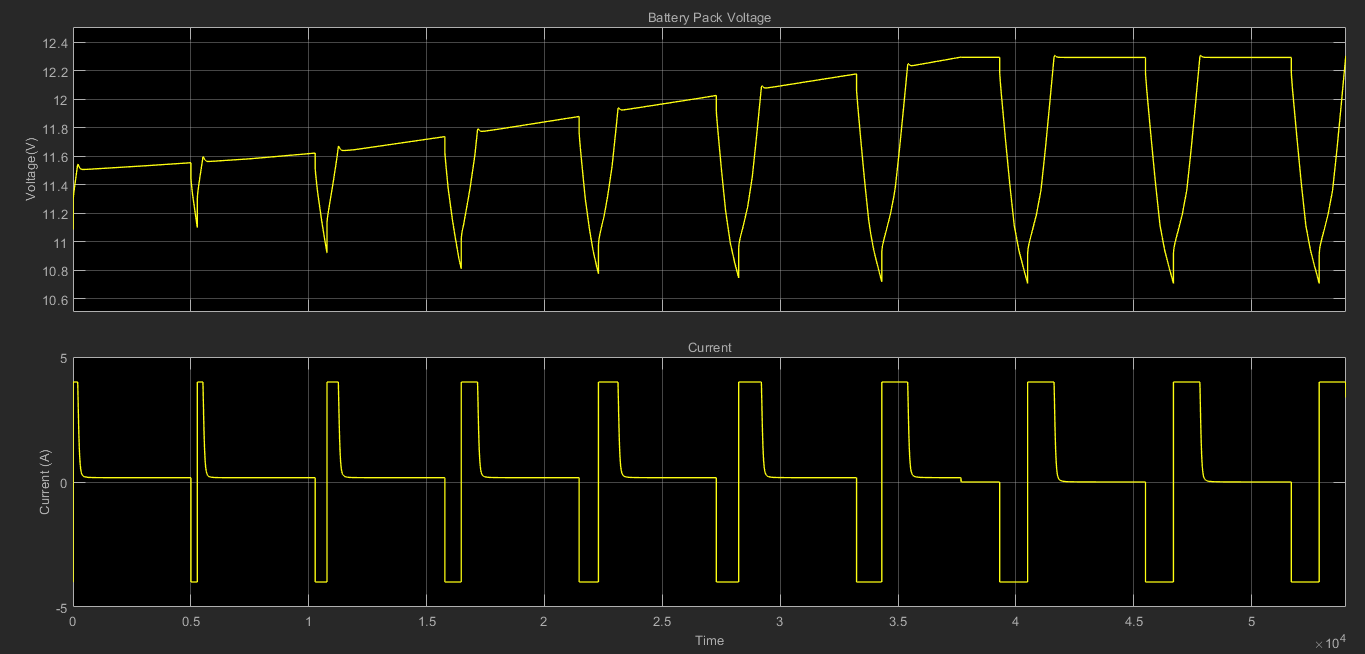
\includegraphics[scale = 0.5]{Chapter5/Figures/batterypackvoltage.png}
    \caption{Battery pack voltage and current versus time during charge-discharge cycles}
\end{figure}
\vspace{0.5cm}
Figure 5.3 shows battery pack voltages before and after balancing so it gives an observation that imbalanced circuit will not only affect the effective capacity of battery but also the terminal voltage of the battery pack. And a increase of nearly 0.6V is observed after battery got balanced by the circuit.

\pagebreak

\section{Cell balancing module test results} 
The debugging of the circuit is done using ST-Link Debugger with Keil. And data transaction between the battery monitoring \acrshort{ic} and the microcontroller is monitored in order to verify whether the module and code is working as expected. 

\begin{figure}[H]
    \centering
    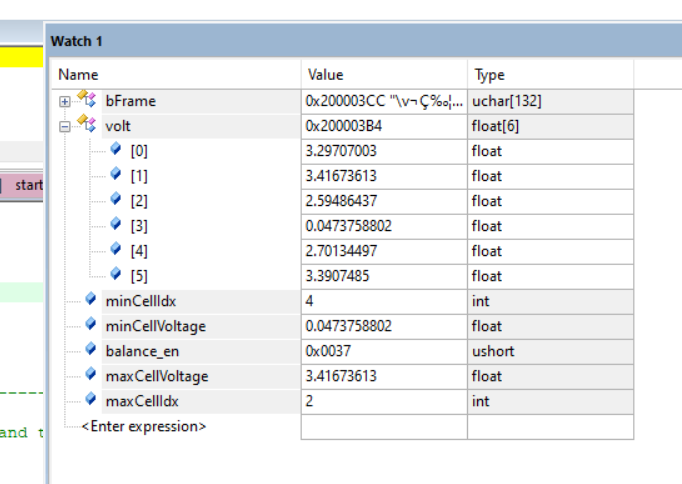
\includegraphics[scale = 0.7]{Chapter5/Figures/Screenshot (68).png}
    \caption{Battery pack voltage readings with minimum and maximum cell voltages}
\end{figure} 

Figure 5.4 shows the watch point in Keil IDE showing all the cell voltages in the battery pack with minimum and maximum cell voltage. 

